\hrulefill 
\section{Sprint 1}

\subsection{Goal}
Lo scopo di questo primo sprint è di realizzare le funzionalità per la registrazione e autenticazione dei clienti e produttori sia lato frontend sia lato backend, l'impostazione del database, la configurazione iniziale dell'ambiente di lavoro e l'implementazione di una semplice interfaccia grafica per la gestione dei prodotti quali l'inserimento ed eliminazione.

\subsection{Sprint Planning}

% \subsubsection{Tabella sprint backlog}

\vspace{-1cm}

\renewcommand{\arraystretch}{2}
\begin{longtable}{p{0.5cm}|p{2.7cm}|p{4.5cm}|p{1.7cm}|p{1.5cm}|p{0.2cm}|p{0.2cm}|p{0.2cm}|p{0.2cm}|p{0.2cm}|p{0.2cm}|p{0.2cm}}
    \caption{Tabella sprint backlog}
    \label{tab:SprintBackLogTableDettagliato} \\
    
    \hline
    \textbf{ID} &\textbf{Nome} & \textbf{Sprint Task} & \textbf{Volontario} & \textbf{Impegno stimato iniziale} & 1 & 2& 3& 4& 5& 6& 7\\
    \hline
    \endfirsthead
    
    \hline
    \textbf{ID} &\textbf{Nome} & \textbf{Sprint Task} & \textbf{Volontario} & \textbf{Impegno stimato iniziale} & 1 & 2& 3& 4& 5& 6& 7\\
    \hline
    \endhead
    
    \multirow{4}{0.2cm}{29} & \multirow{4}{0.2cm}{Creazione database} 
    & Creazione account su MongoDB & Team & 1 & 1& & & & & &\\
    && Creazione database & Cristiano& 1 & 1& & & & & &\\
    && Connessione database & Team & 1 & 1& & & & & &\\
    
    \hline
    
    \multirow{3}{0.2cm}{31} & \multirow{3}{0.2cm}{Creazione reposi\\tory GitHub} 
    & Creazione repo e inizializzazione con NodeJS & Cristiano & 1 & 1& & & & & &\\
    && Installazione dei moduli Node necessari & Cristiano& 1 & 1& & & & & &\\
    
    \hline
    \newpage
    
    \multirow{8}{0.2cm}{14} & \multirow{8}{0.2cm}{Inserimento prodotto} 
    & creazione del modello lato backend & Cristiano & 1 & 1& & & & & &\\
    && creazione modello Produttore lato backend & Cristiano & 1& 1 & & & & & &\\
    && creazione delle API per inserire il prodotto & Cristiano & 3&3 & 3&2 &1 & & &\\
    && creazione delle API per inserire il produttore & Cristiano & 3&3 & 3&2 &1 & & &\\
    && creazione di una semplice interfaccia Vue & Giacomo & 4&4 & 4&3 &2 &1 & &\\
    
    \hline
    
    \multirow{3}{0.2cm}{15} & \multirow{3}{0.2cm}{Rimozione prodotto} 
    & creazione delle API per rimuovere il prodotto & Cristiano & 1 & & & & & & &\\
    && creazione di una semplice interfaccia Vue & Giacomo & 4&4 & 4&3 &2 &1 & &\\
    
    
    \hline
    \multirow{3}{0.2cm}{20} & \multirow{3}{0.2cm}{Aggiornamento prodotto} 
    & creazione delle API per aggiornare il prodotto & Cristiano & 1 & & & & & & &\\
    && creazione interfaccia Vue per la modifica dei dati  & Giacomo & 4&4 & 4&3 &2 &1 & &\\
    
    
    \hline
    
    \multirow{6}{0.2cm}{2} & \multirow{6}{0.2cm}{Autenticazione cliente/produttore } 
    & Studiare come funziona Firebase & Martina & 2&2 & 1& & & & &\\
    && creazione interfaccia Vue per gestire l'autenticazione & Martina & 4&4 & 3& 2& 1& & &\\
    && creazione di API per interagire con l'autenticazione & Martina & 4&4 & 3& 2& 1& & &\\
    && creazione del Token JWT lato backend  & Martina & 4&4 & 3& 2& 1& & &\\
    
    
    \hline
    
    \multirow{6}{0.2cm}{1} & \multirow{6}{0.2cm}{Registrazione cliente/produttore } 
    & creazione delle API per registrare il produttore & Cristiano & 1 & 1 & & & & & &\\
    && creazione delle API per registrare il cliente  & Martina & 1 & 1 & & & & & &\\
    && creazione interfaccia Vue registrazione produttore  & Martina & 4& 4 & 4& 3 &2 &1 & &\\
    && creazione interfaccia Vue registrazione cliente  & Martina & 3& 3 & 2& 2 &2 &1 & &\\
    
    \hline
    
    \multirow{3}{0.2cm}{7} & \multirow{3}{0.2cm}{Visualizza dettaglio} 
    & creazione delle API per leggere un prodotto & Cristiano & 1 & 1 & & & & & &\\
    && creazione interfaccia Vue per visualizzare i prodotti  & Giacomo & 2& 2 & 1& 1 & & & &\\
    
    
    
    
    \hline
    \hline
    \hline
    \multicolumn{4}{r|}{Totale: }& 53&51 &38 & 27&16&8&1&0\\
    \hline
    \multicolumn{4}{r|}{Ideale: }& 53&45 &38 & 30&23&15&8&0\\
    

\end{longtable}

\subsection{Burndown Chart}

\begin{figure}[!ht]
    \centering
    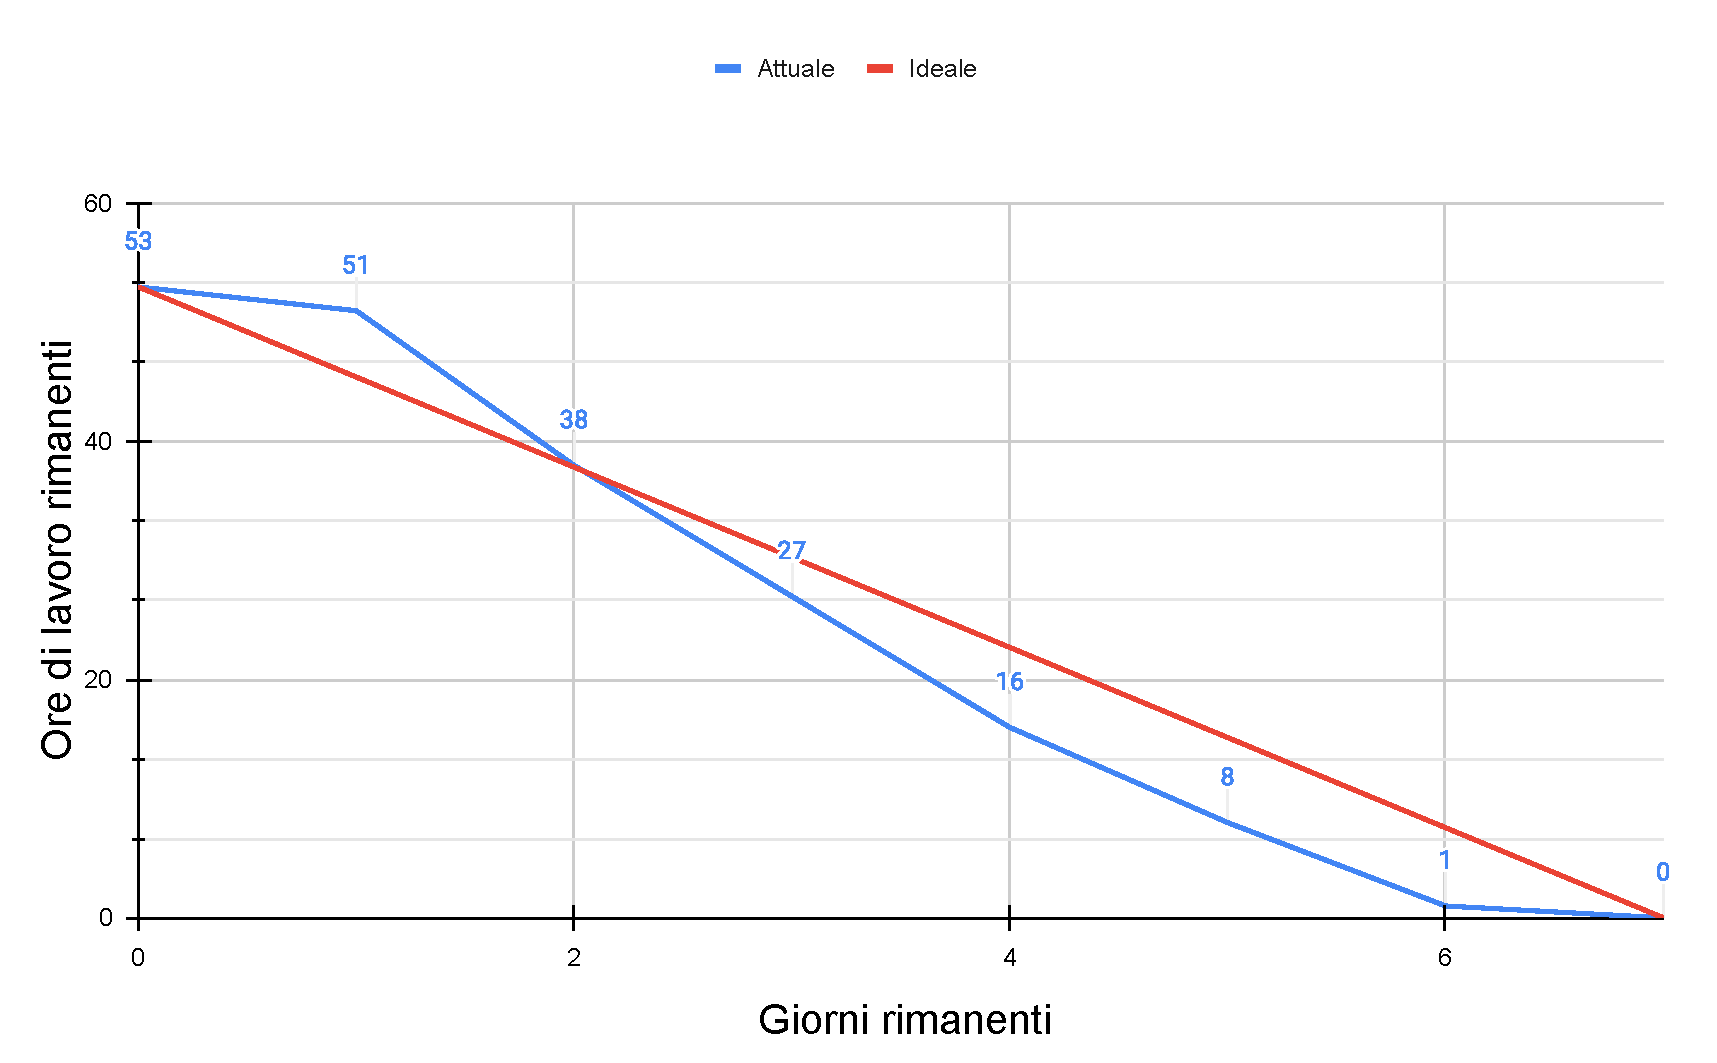
\includegraphics[trim= 0cm 0cm 0cm 0cm, clip, width=1\linewidth]{Deliverables/third-deliverable/img/BurndownChart.pdf}
    \caption{Burndown Chart Sprint \#$1$}
\end{figure}

\restoregeometry

\subsection{Architettura di Progetto e Stack Tecnologico}
Per lo sviluppo del nostro progetto abbiamo implementato un'architettura client-server con comunicazione RESTful. La soluzione è strutturata nei seguenti componenti:

\subsubsection*{Frontend}
    \begin{itemize}
    \item Vue.js 3, framework JavaScript progressivo per la costruzione di interfacce utente moderne e reattive
    \end{itemize}
\subsubsection*{Backend}
    \begin{itemize}
    \item Node.js, ambiente di runtime JavaScript lato server
    \item Express, framework web minimale e flessibile per la gestione delle richieste HTTP e la definizione delle API
    \item MongoDB, database NoSQL orientato ai documenti per la persistenza dei dati
    \end{itemize}
\subsubsection*{Strumenti di sviluppo}
    \begin{itemize}
    \item Axios per gestire le chiamate HTTP tra client e server
    \item MongoDB Compass per la visualizzazione e manipolazione diretta dei dati
    \item Firebase per implementare un sistema di autenticazione sicuro
    \item Git per il controllo di versione e la collaborazione nel team
    \item Postman per il testing delle API
    \item Visual Studio Code come ambiente di sviluppo integrato
    \end{itemize}
La codebase è organizzata secondo una chiara separazione delle responsabilità, con una struttura che distingue modelli (dati), controller (logica applicativa) e router (gestione delle rotte API), garantendo così modularità e manutenibilità del codice.


